\chapter{METODOLOGI}

\section{Metode yang digunakan}

Metode yang akan digunakan dalam penelitian ini terdapat pada gambar \ref{fig:Flowchart}

\begin{figure} [H] \centering
  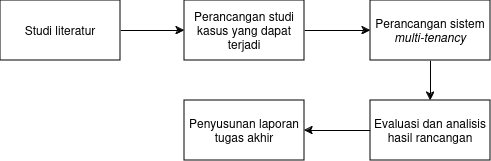
\includegraphics[scale=0.7]{gambar/flowchart.png}
  \caption{Diagram alir implementasi}
  \label{fig:Flowchart}
\end{figure}

\begin{enumerate}
  \item{Studi literatur}
  \par{Pada tahap ini dilakukan studi literatur mengenai konsep dan permasalahan terkait
    dengan \emph{multi-tenancy} pada Kubernetes. Studi literatur dilakukan melalui jurnal penelitian
    yang pernah dilakukan dan juga melalui internet seperti website resmi dari Kubernetes.
  }

  \item{Perancangan sistem \emph{multi-tenancy}}
  \par{Pada tahap ini dilakukan perancangan sistem \emph{multi-tenancy} yang nantinya
    akan diterapkan pada klaster Kubernetes.
  }

  \item{Evaluasi dan analisis hasil rancangan}
  \par{Pada tahap ini dilakukan evaluasi dan analisis dari hasil rancangan yang telah
    dibuat. Evaluasi dan analisis dilakukan untuk mengetahui apakah rancangan yang
    telah dibuat sebelumnya dapat berjalan dengan baik atau tidak. Selain itu, evaluasi
    dan analisis juga dilakukan untuk mengetahui perbedaan implementasi \emph{multi-tenancy}
    yang dapat digunakan pada klaster Kubernetes.
  }

  \item{Penyusunan laporan tugas akhir}
  \par{Tahap ini merupakan tahap terakhir dari penelitian yaitu penyusunan laporan
    dalam bentuk buku tugas akhir yang menjelaskan dasar teori dan metode yang digunakan
    pada tugas akhir serta hasil implementasi yang telah dibuat.
  }
\end{enumerate}

\section{Bahan dan peralatan yang digunakan}

Beberapa peralatan \emph{hardware} dan \emph{software} yang digunakan untuk mendukung pengerjaan
adalah sebagai berikut:
\begin{itemize}
  \vspace{-0.3cm}\item{Laptop Lenovo Legion 5i}
  \vspace{-0.3cm}\item{\emph{Tools} untuk membuat klaster lokal seperti Kind, Minikube, k3s, dan k3d}
  \vspace{-0.3cm}\item{Vagrant untuk membuat \emph{virtual machine}}
\end{itemize}

\section{Urutan pelaksanaan penelitian}

Urutan pelaksanaan penelitian yang akan dilakukan terdapat pada gambar \ref{fig:flowchart_pelaksanaan}
berikut:

\begin{figure} [H] \centering
  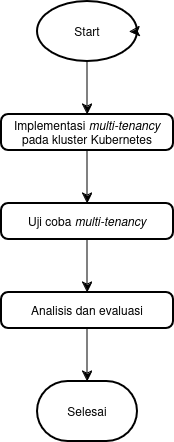
\includegraphics[scale=0.7]{gambar/flowchart_pelaksanaan.png}
  \caption{Diagram alir pelaksanaan}
  \label{fig:flowchart_pelaksanaan}
\end{figure}

Untuk waktu pelaksanaan penelitian terdapat pada tabel \ref{tbl:timeline} berikut:

\begin{table}[H]
  \begin{tabular}{|p{3.5cm}|c|c|c|c|c|c|c|c|c|c|c|c|c|c|c|c|}
    \hline
    \multirow{2}{*}{Kegiatan} & \multicolumn{16}{|c|}{Minggu}                                                                       \\
    \cline{2-17}              &
    1                         & 2                             & 3  & 4  & 5  & 6  & 7  & 8  & 9  & 10 & 11 & 12 & 13 & 14 & 15 & 16 \\
    \hline

    Studi literatur           &
    \G                        & \G                            & \G & \G & \w & \w & \w & \w & \w & \w & \w & \w & \w & \w & \w & \w \\
    \hline

    Perancangan sistem \emph{multi-tenancy} &
    \w                        & \w                            & \w & \w & \G & \G & \G & \G & \w & \w & \w & \w & \w & \w & \w & \w \\
    \hline

    Evaluasi dan analisis hasil rancangan &
    \w                        & \w                            & \w & \w & \w & \w & \w & \w & \G & \G & \G & \G & \w & \w & \w & \w \\
    \hline

    Penyusunan laporan tugas akhir &
    \w                        & \w                            & \w & \w & \w & \w & \w & \w & \w & \w & \w & \w & \G & \G & \G & \G \\
    \hline
  \end{tabular}
  \captionof{table}{Tabel timeline}
  \label{tbl:timeline}
\end{table}
